\subsection{Camera-derived inverse problems and complete cost}

The Huber study uses a camera image resized to $8\times8$ or $16\times16$, with $n=64$ or $256$ unknowns and $4n$ synthetic measurements. The sensing matrix has independent Gaussian entries scaled by $1/\sqrt{4n}$; the positive variant takes their absolute values. The mirror diagonal spans $[1,16]$. Observations are noiseless, $b=Ax_*$, so the minimum objective is zero. These are controlled camera-derived inverse problems, not a benchmark of naturally corrupted measurements. Both sensing variants are retained.

The first positive-sensing blocks at $n=64$ discover horizons $392$, $366$, and $386$ on the three seeds. Each uses one map and one tangent action. Independent replay disagrees by at most $8.6\times10^{-12}$ in absolute whitened dual norm. At $n=256$, the corresponding discovered horizons are $838$, $831$, and $821$, with maximum absolute replay error $3.7\times10^{-11}$. These are exact-arithmetic drift skips verified numerically; the long horizon is determined by the first feature event.

For the complete solve, the certified method tries depths $2,4,8$, caps horizons at $4096$, and requires the bound in \eqref{eq:piecebound} to be at most $0.02\norm{Qc_m}$. It takes sixteen ordinary steps after an unprofitable acquisition. The target is an objective-gap ratio of $10^{-3}$, checked every sixteen work units. Three seeds and three shuffled timing repeats per seed are used on the M4 Mini with one BLAS thread. Timings include discovery, boundary checks, unsuccessful attempts, and objective checks, but exclude matrix setup. All methods reach the target on all seeds in this study.

\begin{table}[htbp]\centering\small

\begin{tabular}{lr rrrr}\toprule

Sensing & $n$ & Ordinary & Fixed & Discovered & Anderson\\\midrule

Positive & 64 & 94.26 & 73.50 & 104.73 & 21.87\\

Signed & 64 & 8.67 & 7.05 & 48.77 & 5.10\\

Positive & 256 & 3002.11 & 1218.88 & 878.85 & 135.01\\

Signed & 256 & 72.87 & 30.48 & 155.87 & 14.45\\

\bottomrule\end{tabular}

\caption{Complete solve milliseconds, median of the per-seed timing medians. Fixed means depth four/horizon sixteen with one settling step. Discovered means the affine-piece certificate.}

\label{tab:discovery}\end{table}

At $n=256$ with positive sensing, the discovered method is 3.47$\times$ faster than ordinary iteration and 1.42$\times$ faster than the fixed finite schedule, using paired per-seed median time ratios. At $n=64$ its acquisition overhead prevents an overall speedup. On signed sensing, frequent piece events make this certificate costly and the discovered method is slower at both sizes. Anderson wins the complete solves here after the initial constant-drift phase ends. The proved local drift obstruction therefore does not imply an end-to-end ranking.

The full solve also exposes a stability distinction hidden by final runtime alone. On positive-sensing seeds zero and one at $n=256$, Anderson reaches recorded objective gaps $25.26$ and $7.35$ times the initial gap before recovering. The certified transport has no comparable excursion at the recorded checkpoints. Checks occur every sixteen work units, so this is not a bound on all intermediate gaps or a claim of monotonicity for approximate certified proposals.

Measurements from the initial scalar implementation of the reduced-path checks are retained as protocol v1. Protocol v2 uses block doubling for $c_j$ and batched feature tests without changing mathematical admission conditions. Both raw records remain available; v2 is used in Table~\ref{tab:discovery}.

\begin{figure}[htbp]\centering

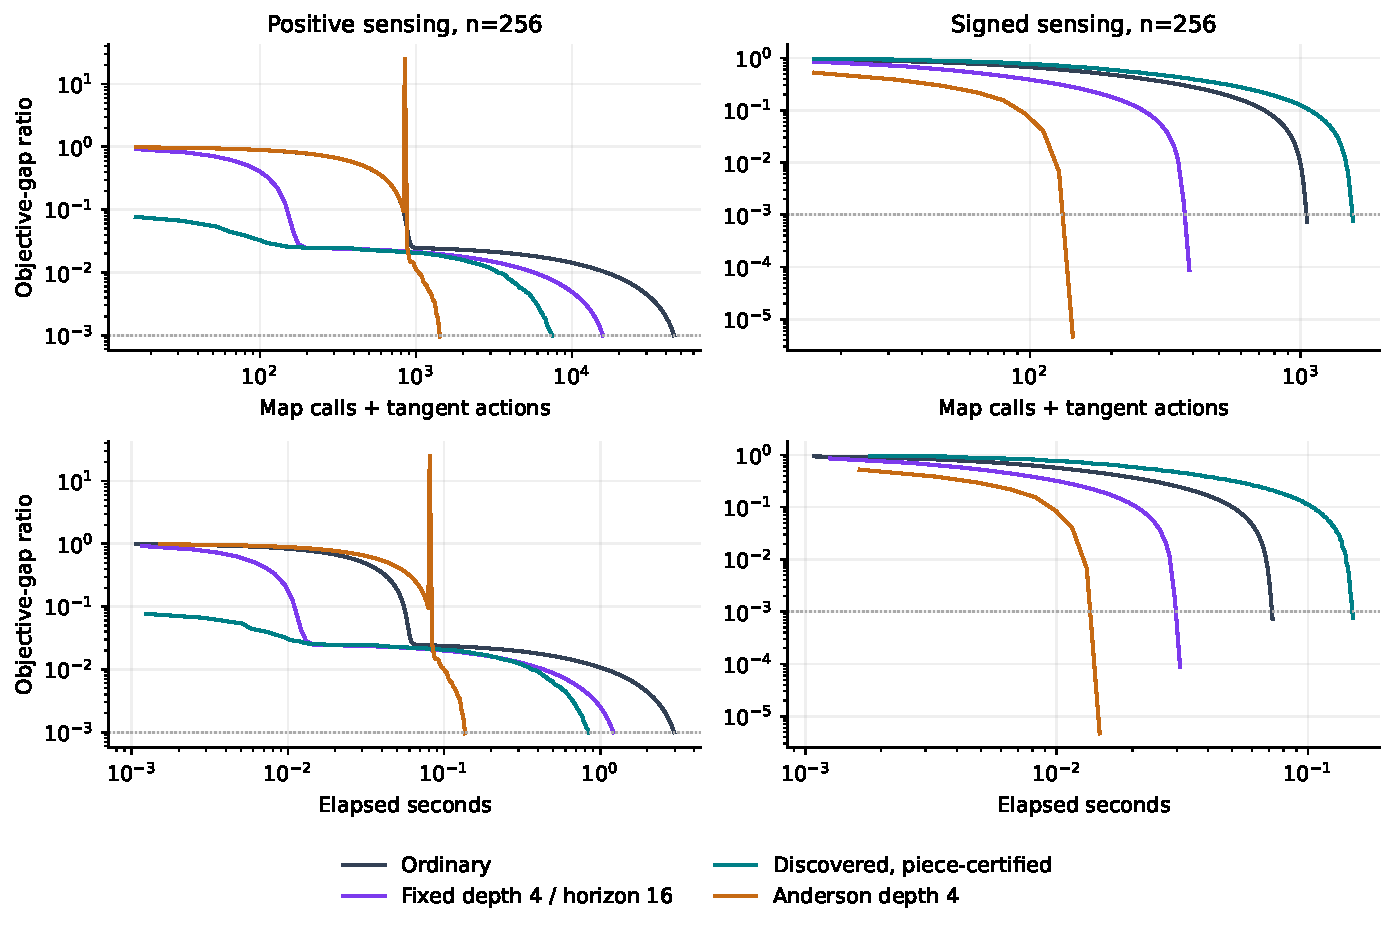
\includegraphics[width=\textwidth]{figures/discovery_costs.pdf}

\caption{Huber mirror descent at $n=256$, seed zero, first timed repeat. The same camera source and target tolerance are used for positive and signed sensing. A discovered valid polynomial can save work and time, while frequent boundary changes can eliminate that benefit. The timing table retains all seeds and repeats.}

\end{figure}

This extension establishes a discoverable, checkable finite transport construction for a nontrivial convex mirror class. The central unresolved problem is to discover comparably economical validity descriptions for curved proximal geometry and changing observable spaces, including the original coupled Meyer iteration.
